\documentclass[12pt, varwidth, border=5mm]{standalone}
\usepackage{tikz}
\usepackage{amsmath}
% Underlining package
\usepackage{ulem}
\usetikzlibrary{calc}
% \usepackage[a4paper, portrait, margin=1cm]{geometry}

\begin{document}
\section*{ }
    \begin{minipage}{0.55\textwidth}
  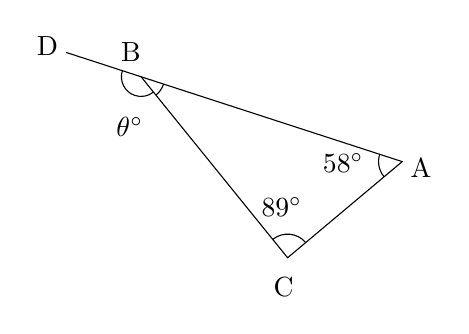
\begin{tikzpicture}[scale=1.0, baseline=(current bounding box.north)]

      \begin{scope}[rotate=162]
        \coordinate (A) at (0,0);
        \coordinate (B) at (3.4866910431520584,0);
        \coordinate (D) at (4.486691043152058,0);
        \coordinate (C) at (intersection cs: first line={(A)--($(A)+(58:4cm)$)}, second line={(B)--($(B)+(180-33:4cm)$)});
        \draw (A) -- (B) -- (C) -- cycle;
        \draw (B) -- (D);

        % Mark angles with arcs
        \draw ($(A)!0.3cm!(B)$) arc [start angle=0, end angle=58, radius=0.3cm];
        \draw ($(B)!0.3cm!(C)$) arc [start angle=180-33, end angle=180, radius=0.3cm];
        \draw ($(C)!0.3cm!(A)$) arc [start angle=180+58, end angle=360-33, radius=0.3cm];
        \draw ($(B)!0.25cm!(D)$) arc [start angle=0, end angle=180-33, radius=0.25cm];

        % Label angles
        \node at ($(A)!-0.25cm!(B)$) {A};
        \node at ($(B)!-0.50cm!(C)!0.2cm!(A)$) {B};
        \node at ($(C)!-0.25cm!(A)!-0.25cm!(B)$) {C};
        \node at ($(D)!-0.25cm!(A)$) {D};

        % Mark angles in degrees
        \coordinate (midBC) at ($(B)!0.5!(C)$);
        \node at ($(A)!0.75cm!(midBC)$) {$58^\circ$};

        \coordinate (midAC) at ($(A)!0.5!(C)$);
        \node at ($(B)!0.65cm!(midAC)$) {};

        \coordinate (midAB) at ($(A)!0.5!(B)$);
        \node at ($(C)!0.65cm!(midAB)$) {$89^\circ$};

        \coordinate (midDC) at ($(D)!0.3!(C)$);
        \node at ($(B)!0.65cm!(midDC)$) {$\theta^\circ$};

      \end{scope}
    \end{tikzpicture}
\end{minipage}%
\hfill
\begin{minipage}{0.4\textwidth}
    \begin{align*}
      \angle \text{DBC} &= \angle \text{A} + \angle \text{C} \\
      &= 58^\circ  + 89^\circ \\
      &= 147^\circ
    \end{align*}
\end{minipage}

\end{document}
